%!TEX root = ./thesis.tex
%****************************************************************
% preamble only for part II 
%****************************************************************

% change the time name for chapters of the part 2
\renewcommand{\chaptertitlename}{PAPER} 
\renewcommand\thechapter{\Alph{chapter}}
\renewcommand{\chaptername}{Paper}
\renewcommand\thesection{\arabic{section}}
% below renewcommands only useful if you use subimport
\renewcommand{\thetable}{\arabic{table}}
\renewcommand{\thefigure}{\arabic{figure}}
\renewcommand{\thesubtable}{\arabic{subtable}}
\renewcommand{\thesubfigure}{\arabic{subfigure}}
\renewcommand{\theequation}{\arabic{equation}}

% change style for the table of contents of the part 2
\titlecontents{chapter}% <chapter-type>
  [4.8em]% <left>
  {\vspace*{1em}\bfseries\normalsize}% <above-code>
  {\hspace*{-4.8em}Paper~\thecontentslabel:\quad}% <numbered-entry-format>
  {}% <numberless-entry-format>
  {\normalsize\hfill\contentspage}% <filler-page-format>


% if you attach pdf files directly, use \pagestyle{pdfpapers}
% for compiled papers with \subimport, use \pagestyle{compiledpapers}, see % example Paper IV
\pagestyle{pdfpapers} 
%****************************************************************
% Paper I
%****************************************************************
% adjust the position of the bluebox of each chapter if you have OCD like me
\renewcommand{\boxsizept}{60pt} 
\chapter{Scientific Paper I}
\thispagestyle{empty}

\noindent List of authors\vspace{3ex}

\noindent \textit{In \Proc \IntlConf \ldots} \textbf{LNCS}, 035303 (2017)

% the note below please check and comment out later 
\hspace{10cm}
\notes[inline]{
    About how you can attach you publications,
    the \href{https://www.hvl.no/contentassets/14ac5045c88248ffa1cf8c4927111040/hvl-avhandling.dotx}{HVL
    PhD thesis Word template} (page 11) on the HVL website states: 
    "Publiserte artikler kan settes inn i avhandlingen slik de er publiserte og trenger ikke konverteres til denne malen."

    If you want to directly attach original publications (with original publishers' format pdf files), 
    you only need to use "includepdf", but you might need to check the copyright of 
    your publications about republishing.
    However, if you don't want to attach pdf files directly but prefer to recompile 
    your Latex files for previous papers, then just can use "subimport".   
    You can ask doctoral adviser Prof. Håvard Helstrup and your supervisors to get 
    their opinions for which way is reasonable and how to deal with copyright of 
    your publications.
}
% the end of the note

\cleardoublepage

% include paper pdf file
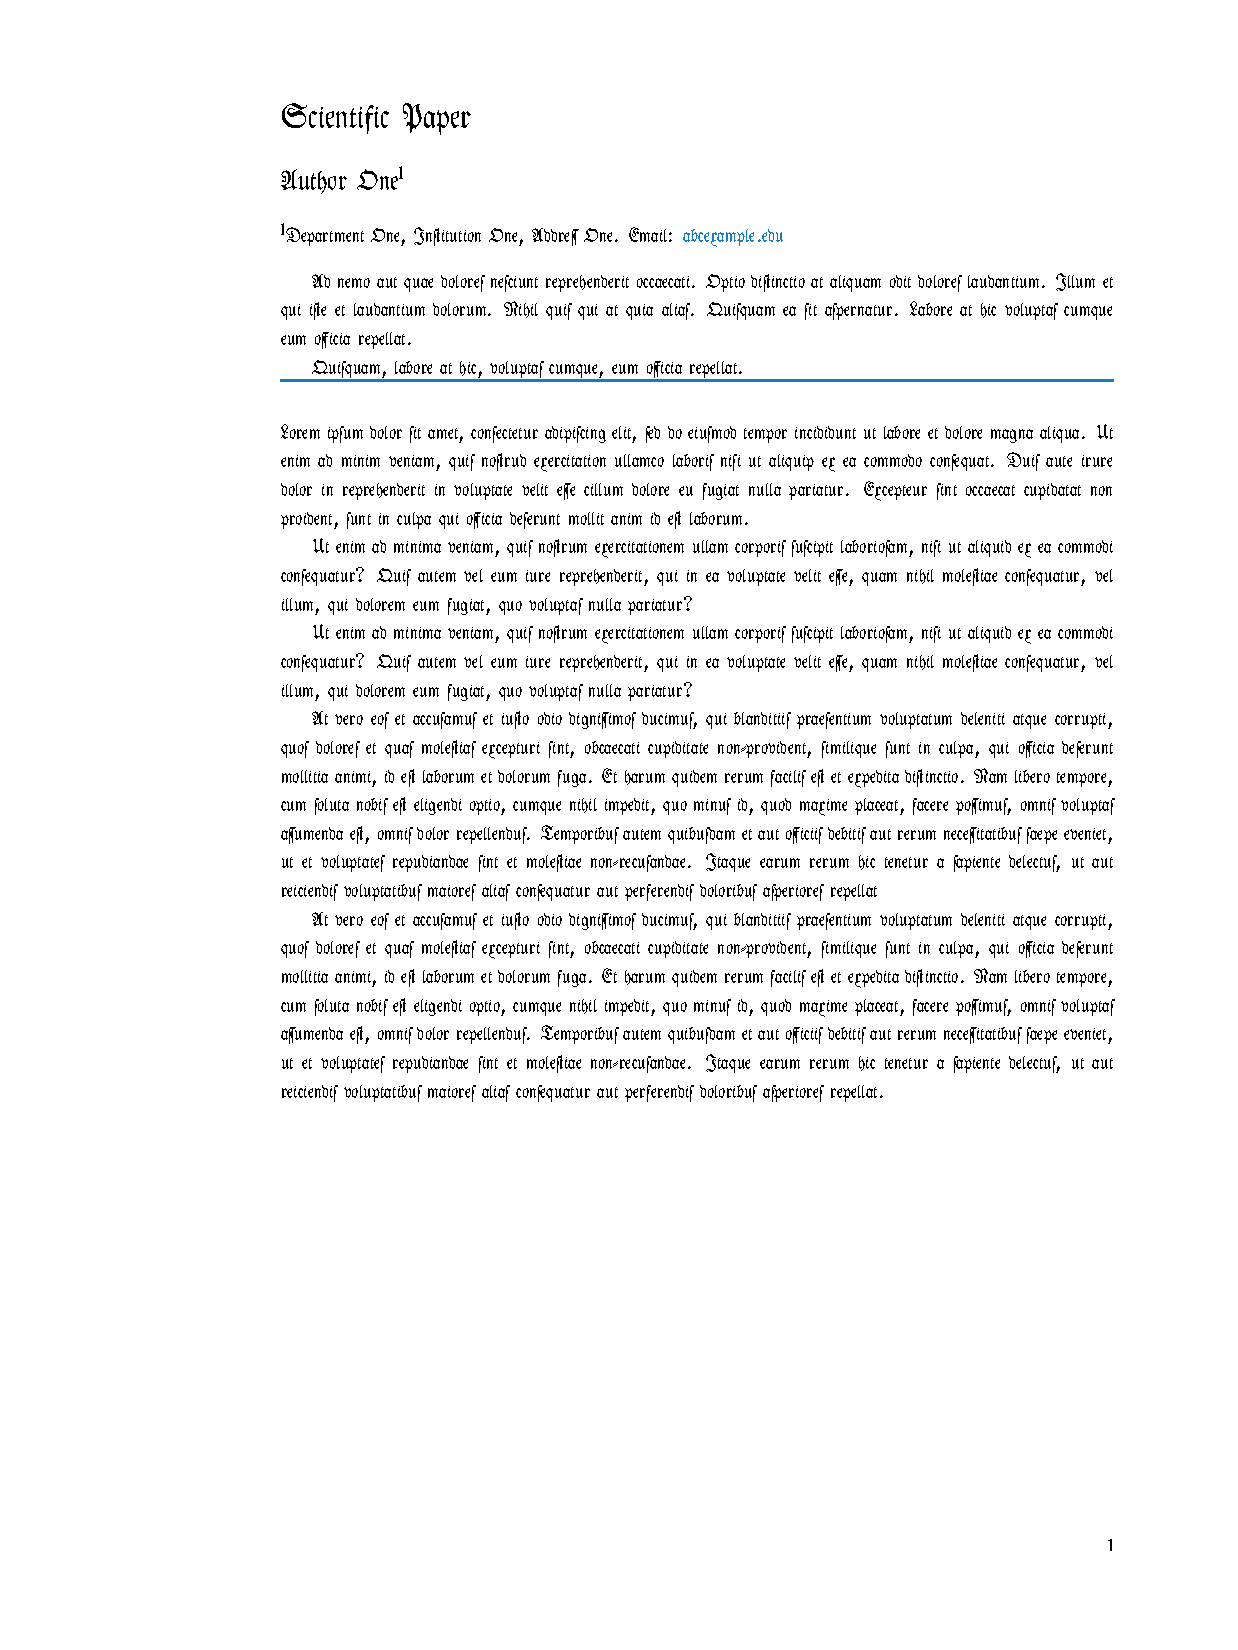
\includepdf[pagecommand=\thispagestyle{plain}, pages=-]{papers/paper1.pdf}

%****************************************************************
% Paper II
%****************************************************************
\renewcommand{\boxsizept}{52pt}
\chapter{Scientific Paper II}
\thispagestyle{empty}

\noindent List of authors\vspace{3ex}

\noindent \textit{In \Proc \IntlConf \ldots} \textbf{IEEE}, 035303 (2017)
\cleardoublepage
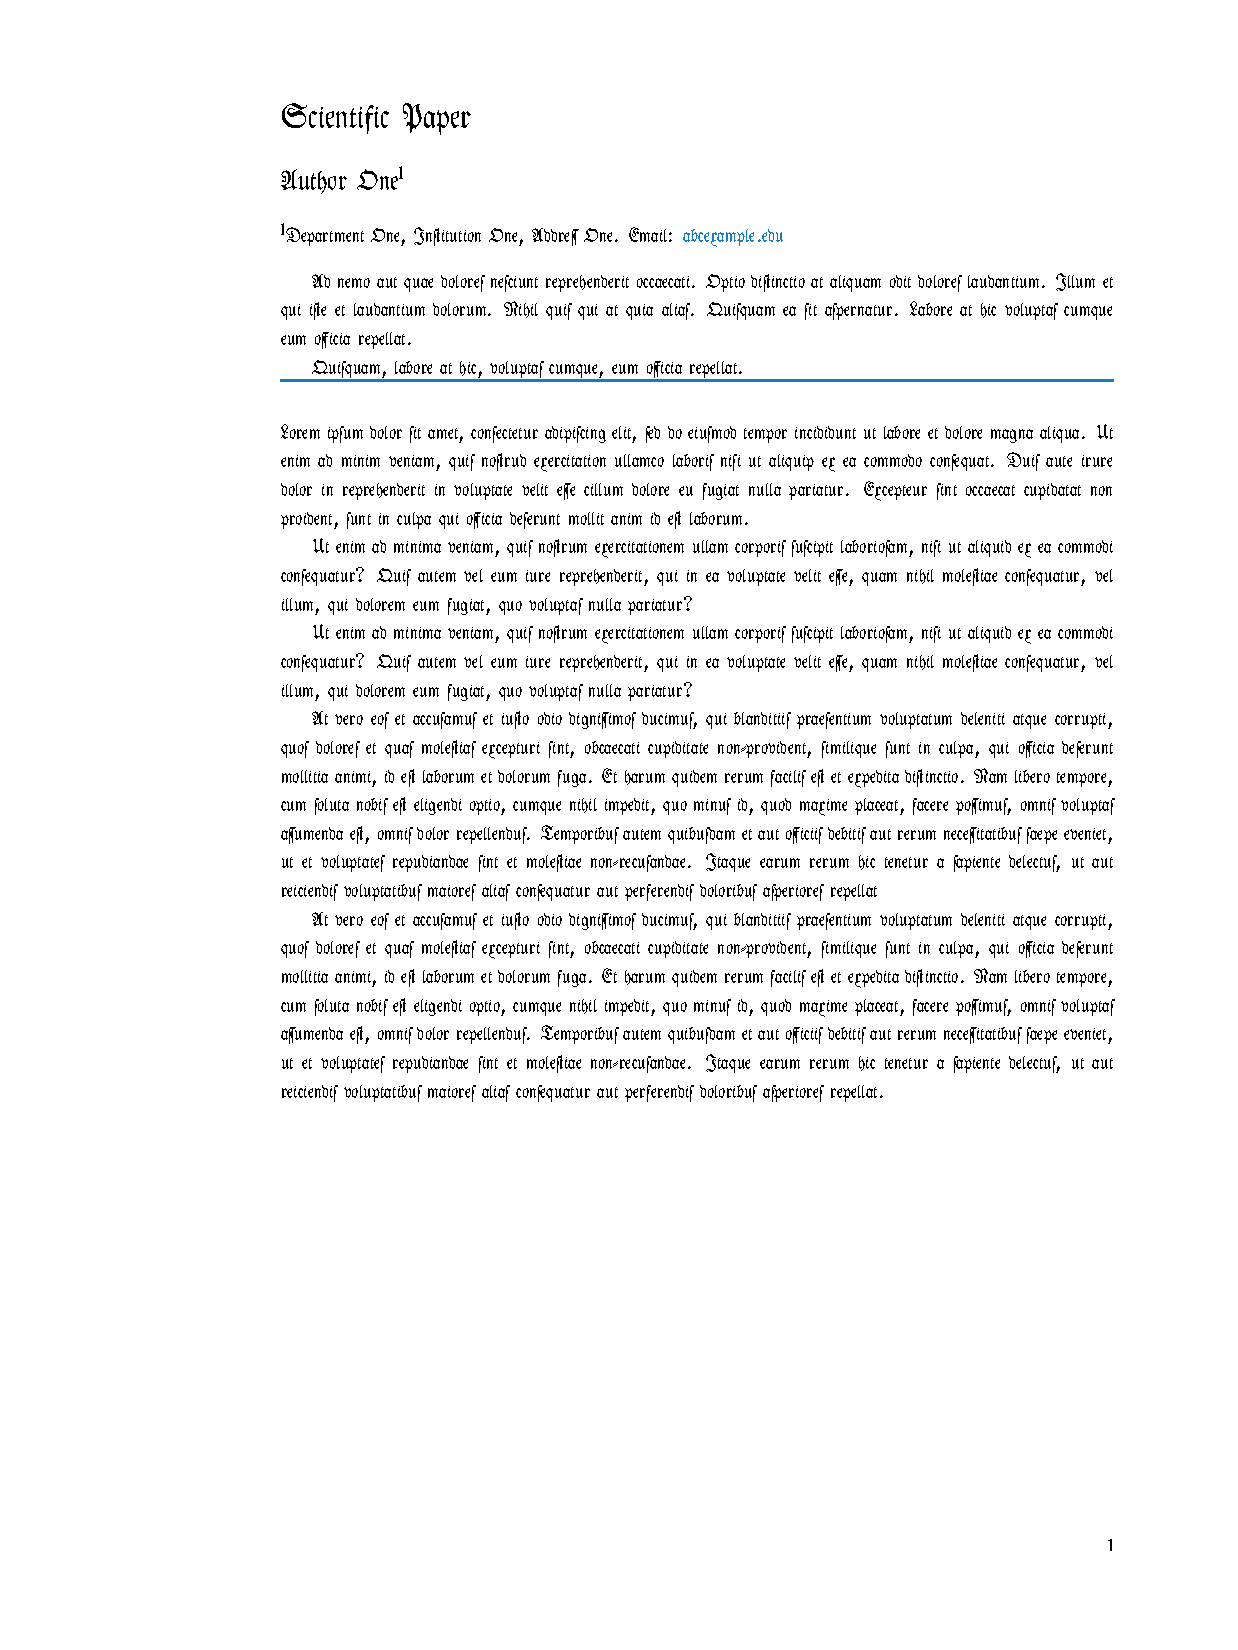
\includepdf[pagecommand=\thispagestyle{plain}, pages=-]{papers/paper2.pdf}

%****************************************************************
% Paper III
%****************************************************************
\renewcommand{\boxsizept}{56pt}
\chapter{Scientific Paper III}
\thispagestyle{empty}

\noindent List of authors\vspace{3ex}

\noindent \textit{In \Proc \IntlConf \ldots} \textbf{IEEE}, 035303 (2017)
\cleardoublepage


%****************************************************************
% Paper IV
%****************************************************************
\renewcommand{\boxsizept}{60pt}

\chapter{Scientific Paper IV}
\thispagestyle{empty}

\noindent List of authors\vspace{3ex}

\noindent \textit{In \Proc \IntlConf \ldots} \textbf{IEEE}, 035303 (2017)
\cleardoublepage

\pagestyle{compiledpapers} % if you use compiled papers with \subimport{}

% the subimport like below to find main.tex in your paper folder,
% the main.tex also needs to be modified to only have \input{} and other useful commands
% (better to make a backup first or make a new branch on you paper repository on Github)
\subimport*{papers/paperdummytex/}{main-dummy.tex}

